\documentclass{article}
\usepackage{amsmath}
\usepackage{amsthm}
\usepackage{amsfonts}
\usepackage{amssymb}
\usepackage{bbold}
\usepackage{dsfont}
\usepackage{graphicx}
\usepackage{cleveref}
\usepackage{bm}
\usepackage{booktabs}
\usepackage{siunitx}
\usepackage{xcolor}
\usepackage[utf8]{inputenc}
\usepackage[english]{babel}
\newtheorem{definition}{Definition}
\newtheorem{example}{Example}
\newcommand{\exP}[1]{\mathrm{e}^{#1}}
\newcommand{\dif}{\mathrm{d}}
\renewcommand{\vec}[1]{\mathbf{#1}}
\newcommand{\pdagger}{{\phantom{\dagger}}}
\newcommand{\state}[1]{\vert #1\rangle}
\newcommand{\cstate}[1]{\langle #1\vert}
\newcommand{\tr}[1]{\mathrm{tr}\left\{#1\right\}}
\newcommand{\trs}[2]{\, \mathrm{tr}_{#1}\{#2\}}
\newcommand{\expc}[3]{\langle #1\vert #2 \vert #3\rangle}
\usepackage[doi=false,url=false,isbn=false,backend=bibtex,style=nature,natbib=true,sorting=none]{biblatex}

\bibliography{bib.bib}

\begin{document}
\title{Energy-space representation of the system-environment coupling: A tight-binding study}
\author{Rudolf Smorka}
\maketitle
\begin{abstract}
	In this document, we discuss how to obtain the energy-representation of the coupling between two one-dimensional tight-binding chains, one describing the 'environment' and the other the 'system'. 
	We show a universal mode-dependency of the coupling between the system modes and the environmental modes, which are inherently linked to the overlap of eigenfunctions across the system-environment interface. The procedure outlined here is valid for a large range of parameters, and we quantify for which coupling strengths our analysis breaks down.
\end{abstract}
\section{The Setup}
We consider two tight-binding chains, one denoted as 'environment'\footnote{Not to be confused with an \textit{infinite} or \textit{thermodynamic} environment, as ours consists of a finite number of sites.} and the other as 'system'. Only the outer most sites of the two chains have a non-vanishing hopping matrix element\footnote{One can think of the setup as being a \textit{single} tight-binding chain with non-uniform hopping amplitudes.}. The Hamiltonian reads
\begin{equation}
	H = H_\mathrm{env} + H_\mathrm{sys} + H_\mathrm{sys-env}
\end{equation}
with the environment tight-binding chain
\begin{equation}
	H_\mathrm{env} = -t_\mathrm{env}\sum_{j=1_\mathrm{env}}^{L_\mathrm{env}-1} d_j^\dagger d_{j+1}^\pdagger +\mathrm{h.c.}
\end{equation}
and the system chain
\begin{equation}
	H_\mathrm{sys} = -t_\mathrm{sys}\sum_{j=1_\mathrm{sys}}^{L_\mathrm{sys}-1} d_j^\dagger d_{j+1}^\pdagger +\mathrm{h.c.}
\end{equation}
For book-keeping reasons we adopt a simple notation, in which each chain is numbered linearly from left to right, starting at their corresponding first site.
Finally, the system-environment coupling is
\begin{equation}
	H_\mathrm{sys-env} = -\gamma d_{L_\mathrm{env}}^\dagger d_{1_\mathrm{sys}}^\pdagger + \mathrm{h.c.},
\end{equation}
so that an electron can hop between the last environment site and the first system site only. 
The Hamiltonian has the following block-structure
\begin{equation}
	H = \begin{pmatrix}
		H_\mathrm{env} & H_\mathrm{sys-env} \\
		H_\mathrm{sys-env}^\dagger & H_\mathrm{sys}
	\end{pmatrix}
\end{equation}
where $H_\mathrm{env}$ and  $H_\mathrm{sys}$ have the usual block tridiagonal structure
\begin{equation}
	T_{L} = \begin{pmatrix}
		0 & 1 & 0 &  0 & \dots & 0\\
		1 & 0 & 1 &  0 &\dots & 0\\
		0 & 1 & 0 & 1 & \dots & 0\\
		
		\vdots &   &  &    &    & \vdots & \\
		0 & 0 & 0 &  \dots& 0  & 1\\
		0 & 0 &  \dots & 0 & 1 &  0
	\end{pmatrix}
\end{equation}
such that $H_\mathrm{env} = -t_\mathrm{env}T_{L_\mathrm{env}}$ and $H_\mathrm{sys} = -t_\mathrm{sys}T_{L_\mathrm{sys}}$. The coupling between the chains has the form
\begin{equation}
	\Gamma_{L,L'} = \begin{pmatrix}
		0 & 0 & \dots & 0\\
		\vdots & & & \vdots\\
		1 & 0 & \dots & 0
	\end{pmatrix} \in \mathds{R}^{L,L'}
\end{equation}
such that $H_\mathrm{sys-env} = - \gamma \Gamma_{L_\mathrm{env},L_\mathrm{sys}}$. Much has been written about the tight-binding model, and we refer here to the literature. 
\section{Partitioned diagonalization}
We now come to the main part of this document. We impose a system-environment separation, similar to the real-space one, in energy-space. This means, that the blocks of $H$ are diagonalized individually
\begin{equation}
	H^\mathrm{p} = \begin{pmatrix}
		U^\dagger H_\mathrm{env} U & A\\
		A^\dagger & V^\dagger H_\mathrm{sys} V
	\end{pmatrix}\label{eq:PartitionedDiagonalization}
\end{equation}
where $A$ is the transformed $L_\mathrm{env}\times L_\mathrm{sys}$ matrix
\begin{equation}
	A = U\Gamma V^\dagger.
\end{equation}
Because we perform with the unitary $U$ of the environment Hamiltonian from the left and with $V^\dagger$ of the system Hamiltonian from the right, $A$ encodes the coupling elements in energy-space. The matrix element $A_{ij}$ encodes the coupling strength of the $i$th environment mode to the $j$th system mode. 
\section{Range of validity of partitioned diagonalization}
When the coupling between the system and the environment becomes too large, it is not possible to perform the partial diagonalization as above. In fact, one cannot distinguish between 'the system' and 'the environment' anymore. In this case, the spectrum of the total Hamiltonian cannot be decomposed into the system and environment spectra. 

We compare this partitioned diagonalization to the full one. Consider the unitary matrix $\Lambda$, which diagonalizes the full hamiltonian $H = \Lambda D\Lambda^\dagger$, with $D$ a diagonal matrix with the spectrum of $H$ as its entries. We impose now, that $\Lambda$ inherits the same block-structure as $H$,
\begin{equation}
	\Lambda = \begin{pmatrix}
		\Lambda_\mathrm{e} & \Lambda_\mathrm{e-s} \\
		\Lambda_\mathrm{e-s}^\dagger & \Lambda_\mathrm{s}
	\end{pmatrix}
\end{equation} 
Performing the diagonalization explicitly, we obtain
\begin{equation}
	\begin{split}
		D &= \Lambda^\dagger H\Lambda \\
		&= \begin{pmatrix}
			\Lambda_\mathrm{e}^\dagger & \Lambda_\mathrm{e-s}^\dagger \\
			\Lambda_\mathrm{e-s} & \Lambda_\mathrm{s}^\dagger
		\end{pmatrix} 
		\begin{pmatrix}
			H_\mathrm{e} & H_\mathrm{e-s} \\
			H_\mathrm{e-s}^\dagger & H_\mathrm{s}
		\end{pmatrix}
		\begin{pmatrix}
			\Lambda_\mathrm{e} & \Lambda_\mathrm{e-s} \\
			\Lambda_\mathrm{e-s}^\dagger & \Lambda_\mathrm{s}
		\end{pmatrix}\\
		&= \begin{pmatrix}
			\Lambda_\mathrm{e}^\dagger H_\mathrm{e} + \Lambda^\dagger_\mathrm{e-s}H_\mathrm{e-s}^\dagger & \Lambda_\mathrm{e}^\dagger H_\mathrm{e-s} + \Lambda^\dagger_\mathrm{e-s}H_\mathrm{s}\\
			\Lambda_\mathrm{e-s} H_\mathrm{e} + \Lambda^\dagger_\mathrm{s}H_\mathrm{e-s}^\dagger & \Lambda_\mathrm{s-e} H_\mathrm{e-s} + \Lambda^\dagger_\mathrm{s}H_\mathrm{s}
		\end{pmatrix}
		\begin{pmatrix}
			\Lambda_\mathrm{e} & \Lambda_\mathrm{e-s} \\
			\Lambda_\mathrm{e-s}^\dagger & \Lambda_\mathrm{s}
		\end{pmatrix}\\
		&= \left(\begin{array}{c|c}
			\Lambda_\mathrm{e}^\dagger H_\mathrm{e}\Lambda_\mathrm{e} + \Lambda^\dagger_\mathrm{e-s}H_\mathrm{e-s}^\dagger\Lambda_\mathrm{e} + & \Lambda_\mathrm{e}^\dagger H_\mathrm{e}\Lambda_\mathrm{e-s} + \Lambda^\dagger_\mathrm{e-s}H_\mathrm{e-s}^\dagger\Lambda_\mathrm{e-s}+  \\
			\Lambda_\mathrm{e}^\dagger H_\mathrm{e-s}\Lambda_\mathrm{e-s}^\dagger + \Lambda^\dagger_\mathrm{e-s}H_\mathrm{s} \Lambda_\mathrm{e-s}^\dagger 
			& \Lambda_\mathrm{e}^\dagger H_\mathrm{e-s}\Lambda_\mathrm{s} + \Lambda^\dagger_\mathrm{e-s}H_\mathrm{s} \Lambda_\mathrm{s}\\ \midrule
			\Lambda_\mathrm{e-s} H_\mathrm{e}\Lambda_\mathrm{e} + \Lambda^\dagger_\mathrm{s}H_\mathrm{e-s}^\dagger\Lambda_\mathrm{e} + & \Lambda_\mathrm{e-s} H_\mathrm{e}\Lambda_\mathrm{e-s} + \Lambda^\dagger_\mathrm{s}H_\mathrm{e-s}^\dagger\Lambda_\mathrm{e-s} +\\
			\Lambda_\mathrm{e-s} H_\mathrm{e-s}\Lambda_\mathrm{e-s}^\dagger + \Lambda^\dagger_\mathrm{s}H_\mathrm{s}\Lambda_\mathrm{e-s}^\dagger &  \Lambda_\mathrm{e-s} H_\mathrm{e-s}\Lambda_\mathrm{s} + \Lambda^\dagger_\mathrm{s}H_\mathrm{s}\Lambda_\mathrm{s}
		\end{array}\right)
	\end{split}\label{eq:FullDiagonalization}
\end{equation}
Comparing \cref{eq:FullDiagonalization} with \cref{eq:PartitionedDiagonalization}, one recognizes, that for the partitioned diagonalization to be valid, the following terms have to vanish
\begin{equation}
	\begin{split}
		\Lambda^\dagger_\mathrm{e-s}H_\mathrm{e-s}^\dagger\Lambda_\mathrm{e} &= 0 \\
		\Lambda^\dagger_\mathrm{e-s}H_\mathrm{s} \Lambda_\mathrm{e-s}^\dagger &= 0\\
		\Lambda_\mathrm{e}^\dagger H_\mathrm{e}\Lambda_\mathrm{e-s} &= 0\\
		\Lambda^\dagger_\mathrm{e-s}H_\mathrm{e-s}^\dagger\Lambda_\mathrm{e-s} &= 0\\
		\Lambda^\dagger_\mathrm{e-s}H_\mathrm{s} \Lambda_\mathrm{s} &= 0\\
		\Lambda_\mathrm{e-s} H_\mathrm{e}\Lambda_\mathrm{e-s} &= 0\\ \Lambda^\dagger_\mathrm{s}H_\mathrm{e-s}^\dagger\Lambda_\mathrm{e-s} &= 0\\
		\Lambda_\mathrm{e-s} H_\mathrm{e-s}\Lambda_\mathrm{s} &= 0
	\end{split}
\end{equation}
Furthermore, the unitary $\Lambda$ diagonalizes $H$, meaning that all other off-diagonal elements have to vanish.\\
\textit{Numerical example}: For $L_\mathrm{env} = 491$, $L_\mathrm{sys}=9$, and $t_\mathrm{env} = 10, t_\mathrm{sys}=1, \gamma = 1$, we show the upper right block of $D$ in \cref{eq:FullDiagonalization} except the part $\Lambda_\mathrm{e}^\dagger H_\mathrm{e-s}\Lambda_\mathrm{s}$ in \cref{fig:RightBlock}. We show the same matrices for $\gamma=12$ in \cref{fig:RightBlock_g12}. 
\begin{figure}[!h]
	\centering
	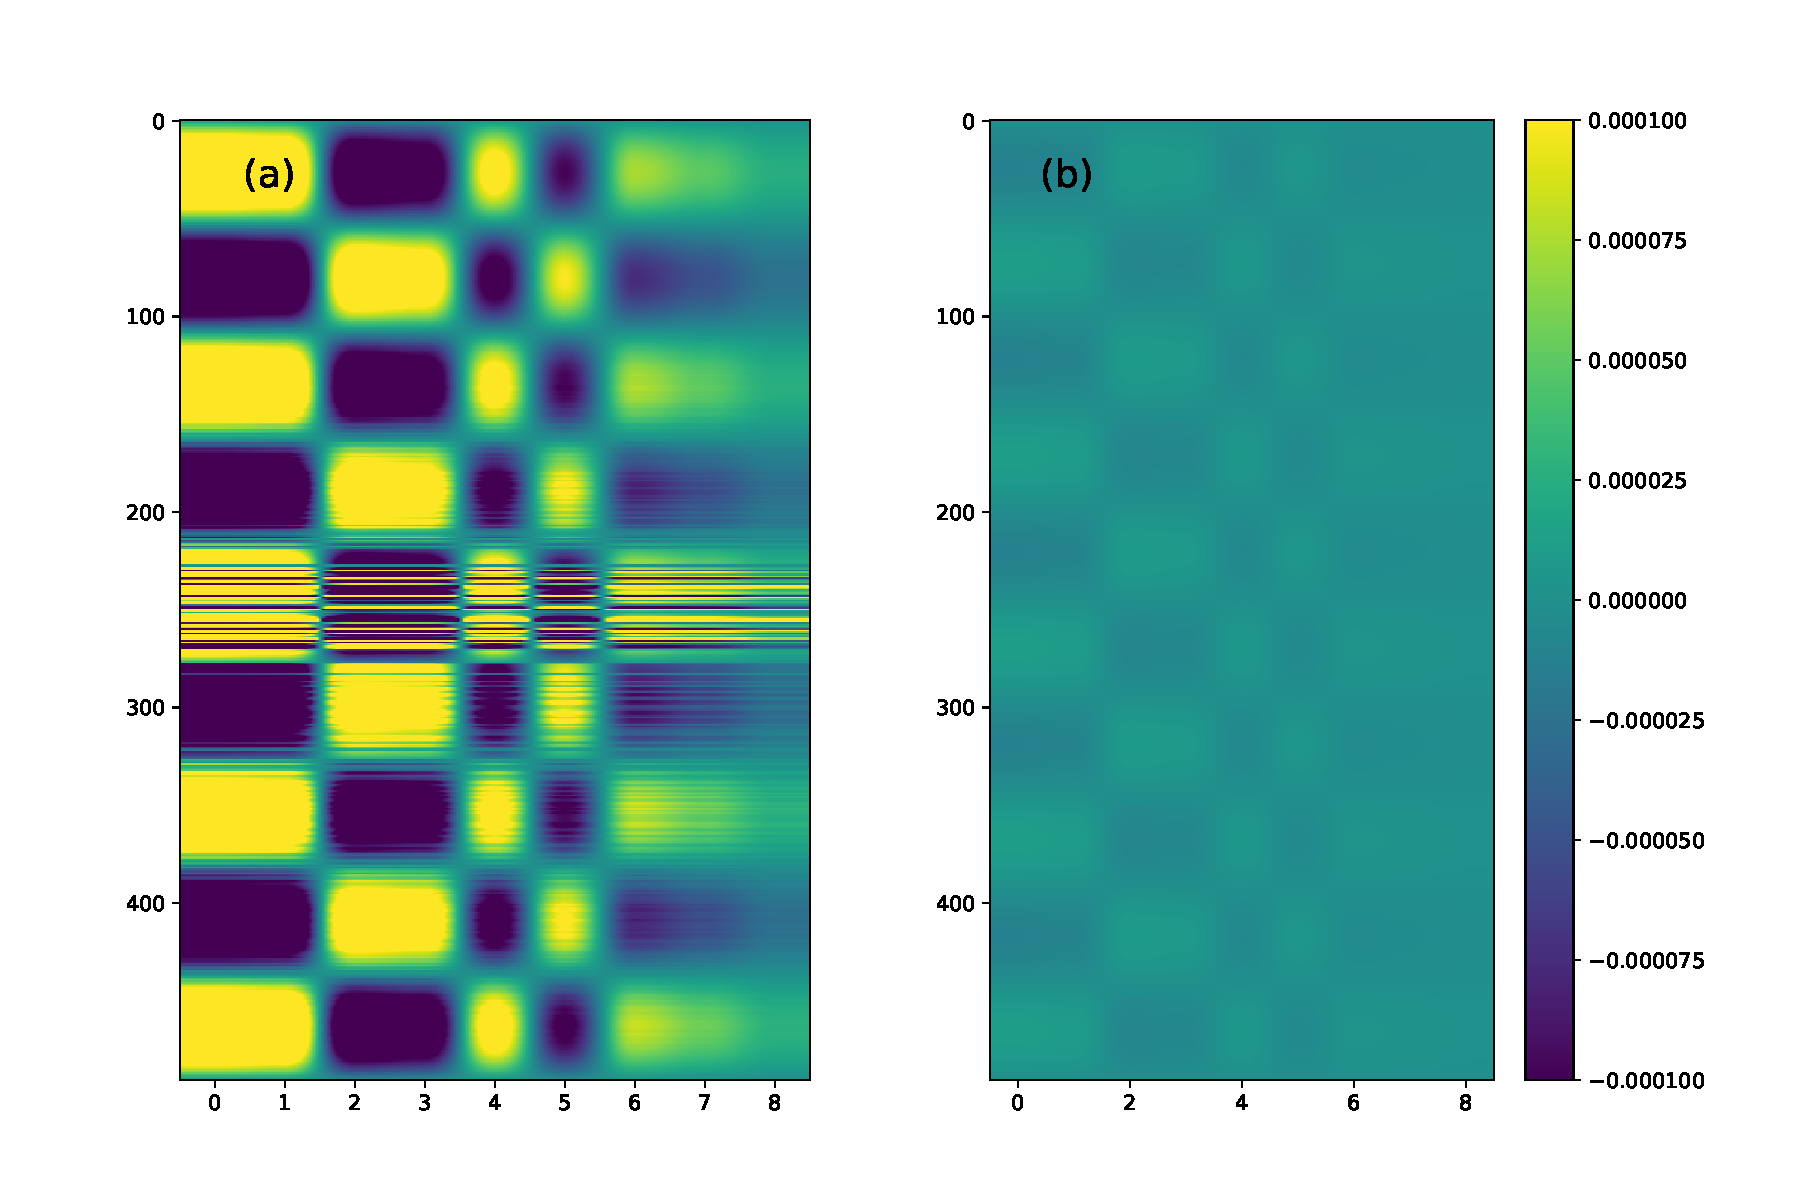
\includegraphics[width=0.8\textwidth]{../plots/RightBlock.pdf}
	\caption{Matrix elements of $\Lambda^\dagger_\mathrm{e} H_\mathrm{e}\Lambda_\mathrm{e-s} + \Lambda^\dagger_\mathrm{e-s} H_\mathrm{e-s}^\dagger\Lambda_\mathrm{e-s} + \Lambda^\dagger_\mathrm{e-s} H_\mathrm{s}\Lambda_\mathrm{s}$ (a) and matrix elements of $\Lambda_\mathrm{e}^\dagger H_\mathrm{e-s}\Lambda_\mathrm{s}$ (b). Parameters are given in the main text.}\label{fig:RightBlock}
\end{figure}\\
\begin{figure}[!h]
	\centering
	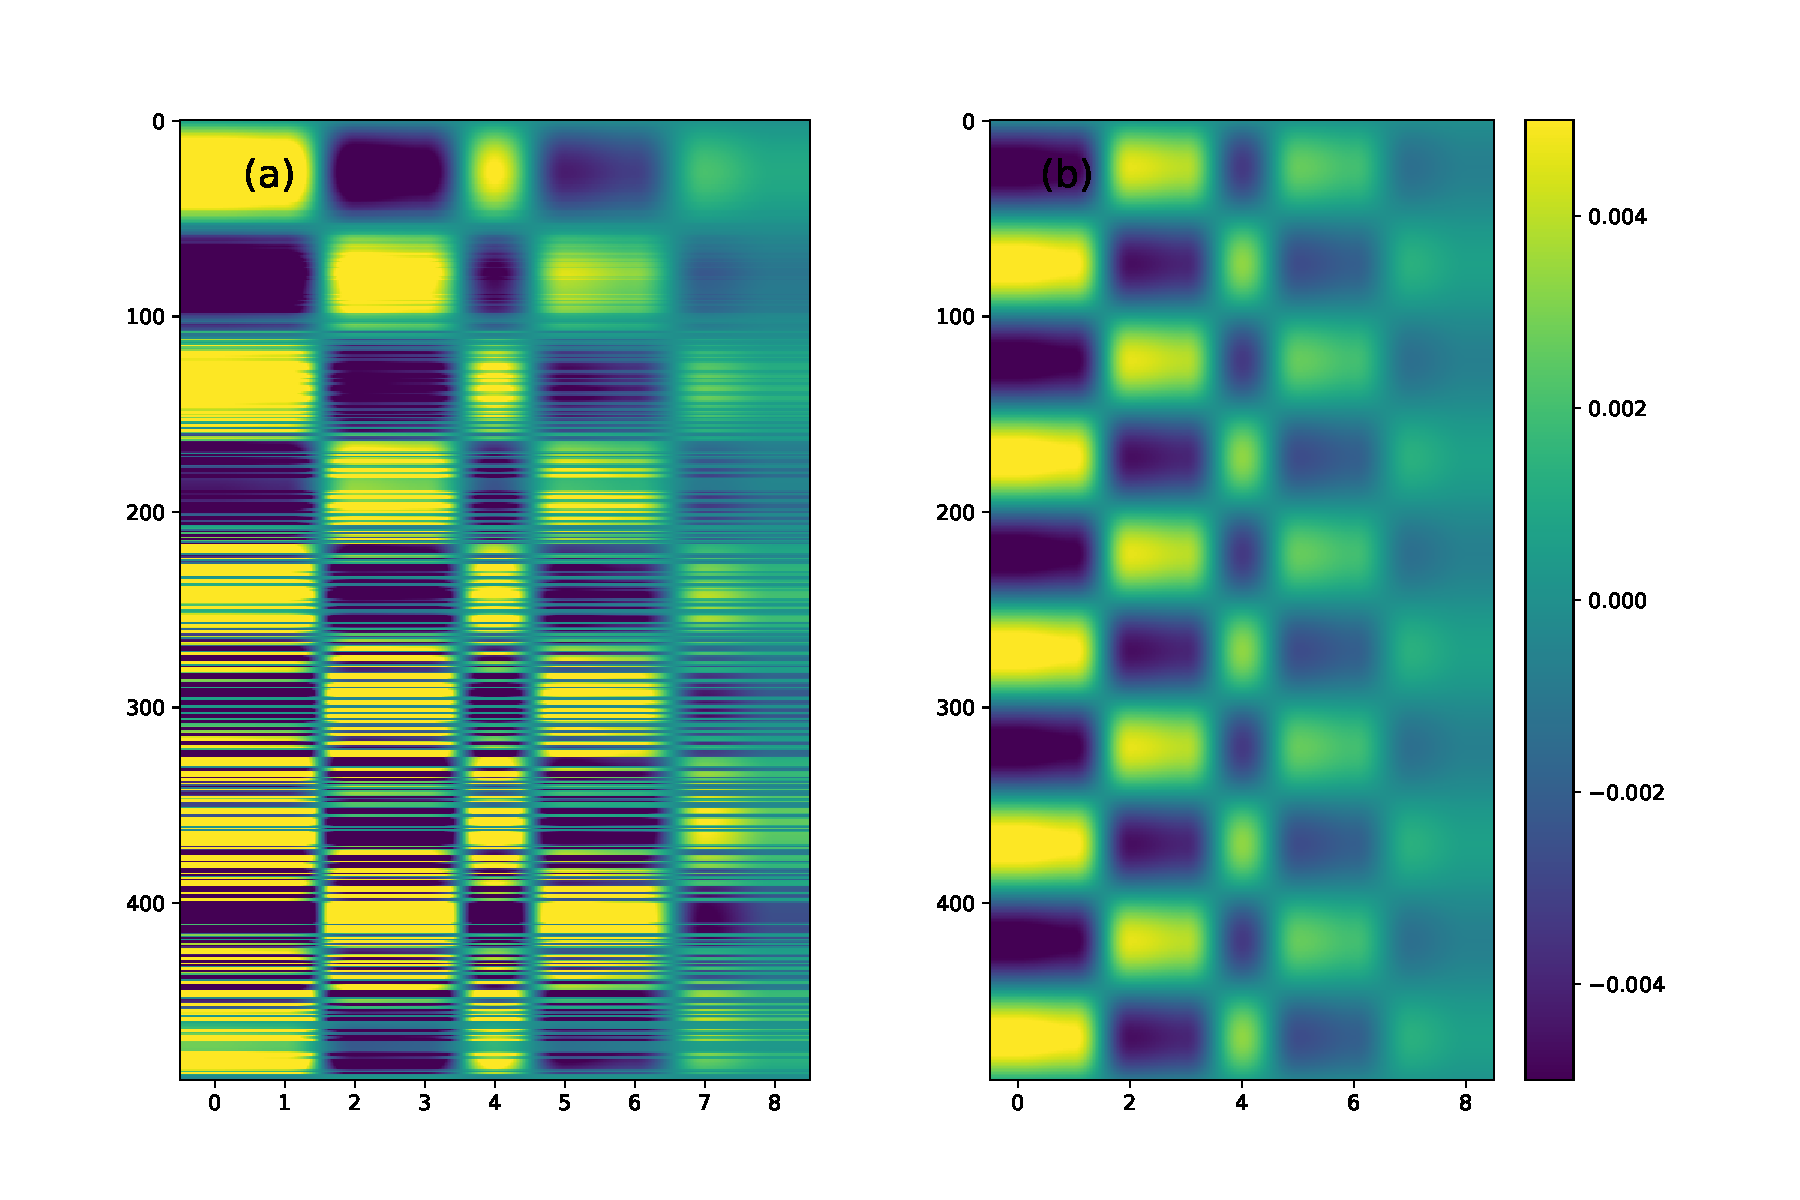
\includegraphics[width=0.8\textwidth]{../plots/RightBlock_g12.pdf}
	\caption{Same as in \cref{fig:RightBlock} but for $\gamma=12$.}\label{fig:RightBlock_g12}
\end{figure}\\
To quantify the degree to which the above analysis is valid, we compare the exact eigenvalues of $H$, $\varepsilon_k$, with the eigenvalues of the partitioned system and environment Hamiltonian $H^\mathrm{p}$, $\varepsilon_k^\mathrm{p}$, using the metric
\begin{equation}
	\eta = \frac{1}{N}\sum_k^N \vert\varepsilon_k - \varepsilon_k^\mathrm{p}\vert.
\end{equation}
For perfect agreement of the partitioned diagonalization and the exact diagonalization, this metric vanishes (because then $\varepsilon_k=\varepsilon_k^\mathrm{p}$). The larger $\eta$, the worse the approximation for the corresponding parameter. In \cref{fig:Eta_Gamma}, we show the dependence of $\eta$ on $\gamma$ for the same parameters as above. The metric $\eta$ remains below $5\times 10^{-14}$ for a wide range of $\gamma$ which indicates that the partitioned diagonalization conserves the spectrum of the full Hamiltonian approximately exactly.
\begin{figure}[!h]
	\centering
	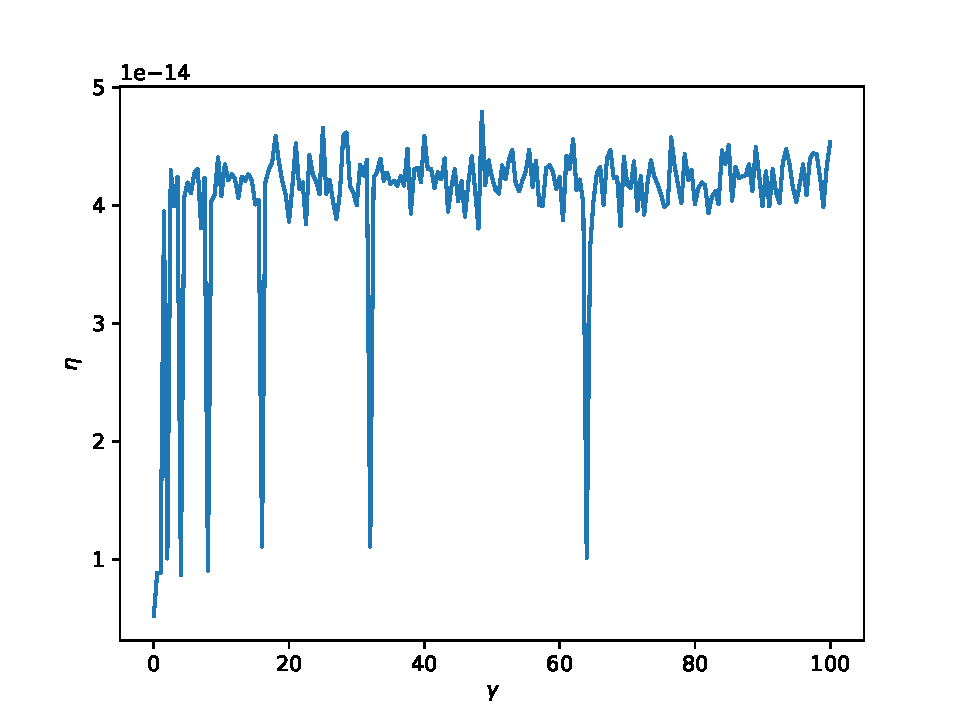
\includegraphics[width=0.7\textwidth]{../plots/Eta_Gamma.pdf}
	\caption{Absolute deviation of eigenvalues using the exact diagonalization and the partitioned diagonalization for various couplings $\gamma$.}\label{fig:Eta_Gamma}
\end{figure}
\section{Energy-dependence of the system-environment coupling}
We now discuss for a specific example the form of $A=U\Gamma V^\dagger$. Again, we consider $L_\mathrm{env} = 491$, $L_\mathrm{sys}=9$, and $t_\mathrm{env} = 10, t_\mathrm{sys}=1$, and $\gamma = 1$. We start with showing the full coupling matrix in $(\varepsilon_\mathrm{env},\varepsilon_\mathrm{sys})$ space in \cref{fig:Coupling_En_full}. From here we can already infer some trends: First, the coupling strength of a single environment mode to all system modes is alternating between positive and negative numbers, and the strength decreases as the system mode energy increases. This can be seen clearly in \cref{fig:Coupling_En_sys}. Second, the coupling of all system states decreases with increasing environment mode energy, meaning that modes near environment Fermi-level couple the strongest to system modes. This can be seen in \cref{fig:Coupling_En_env}
\begin{figure}[!h]
	\centering
	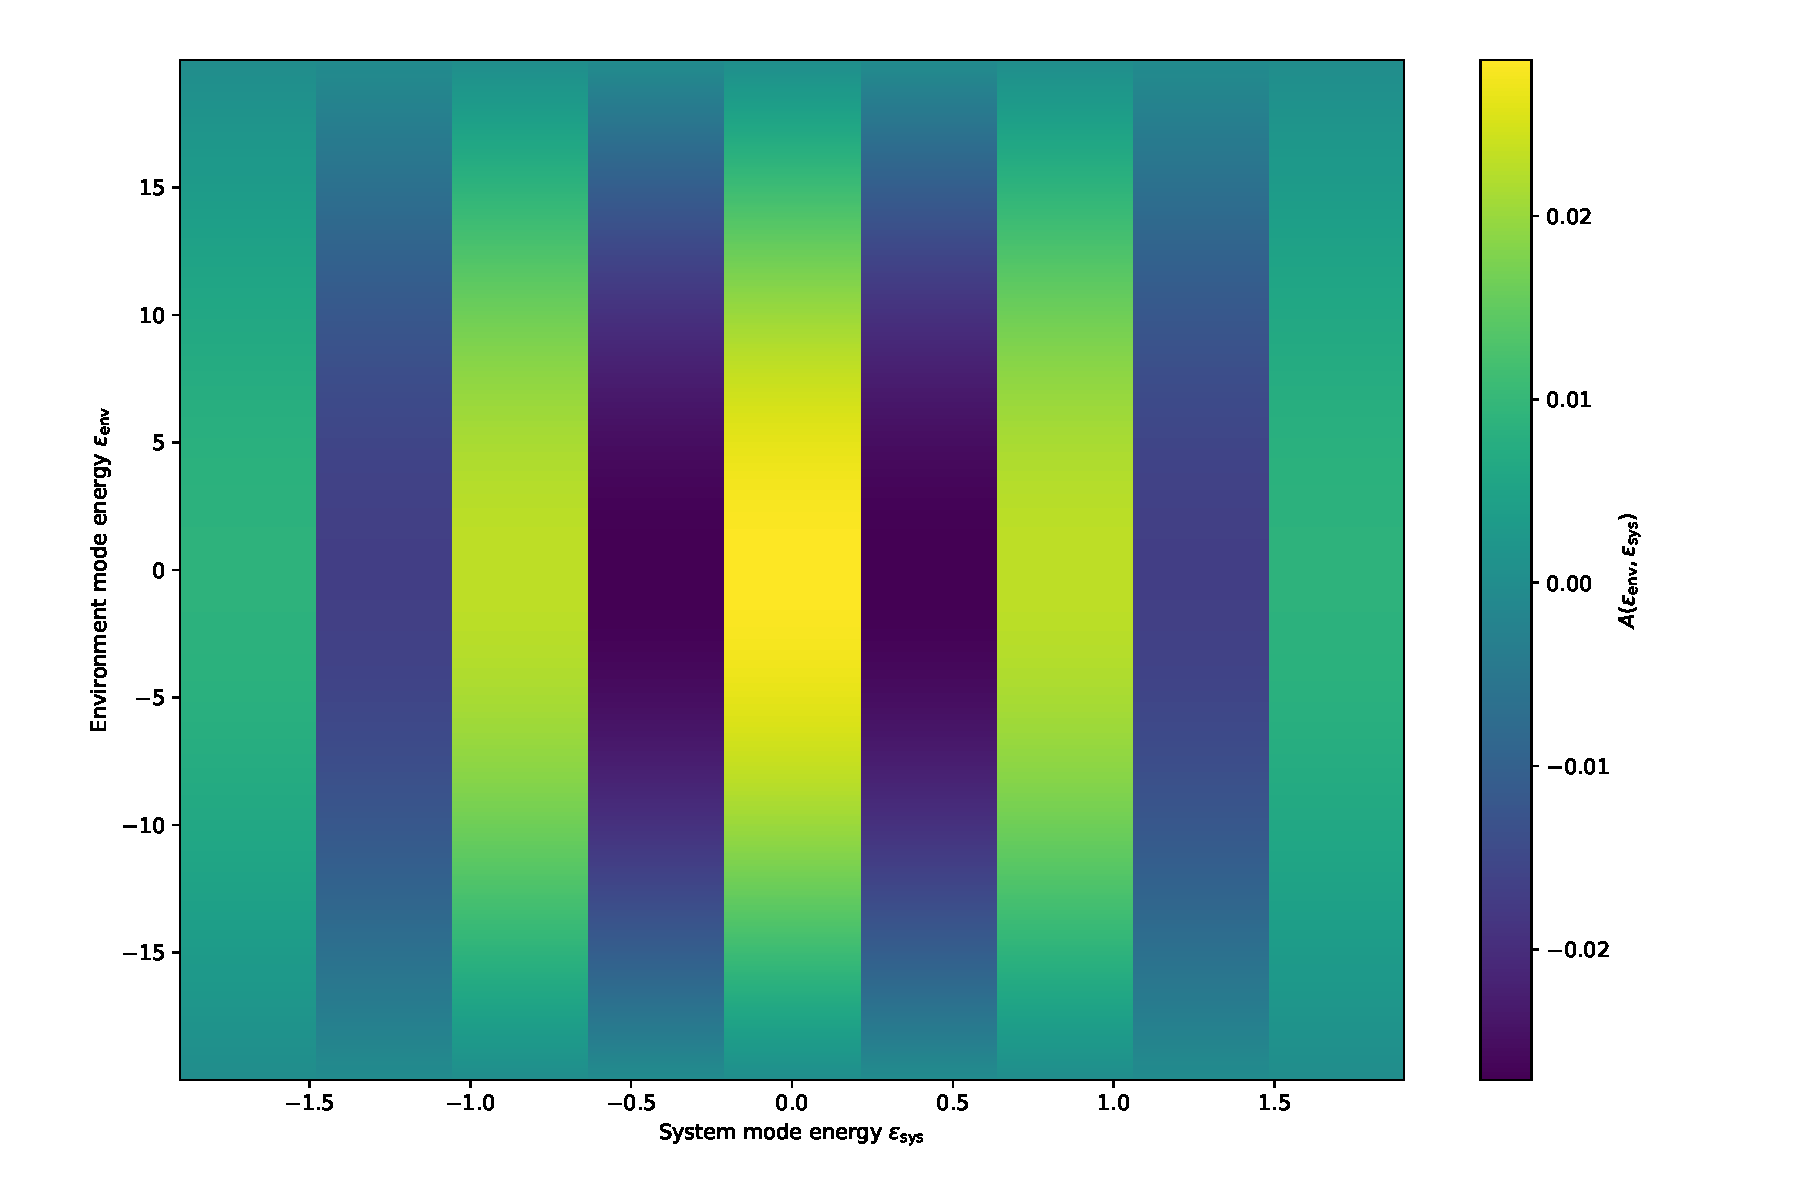
\includegraphics[width=0.9\textwidth]{../plots/Energy_coupling_full.pdf}
	\caption{Full coupling matrix in $(\varepsilon_\mathrm{env},\varepsilon_\mathrm{sys})$ space} \label{fig:Coupling_En_full}
\end{figure}\\
\begin{figure}[!h]
	\centering
	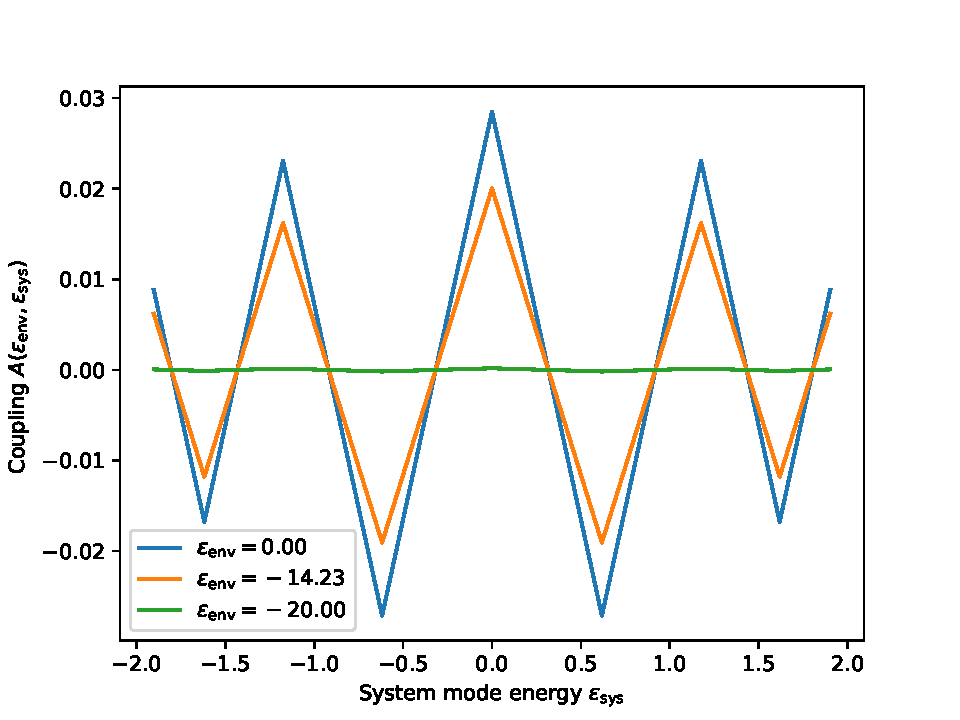
\includegraphics[width=0.9\textwidth]{../plots/Coupling_systemModes.pdf}
	\caption{Coupling of different environment modes to all system modes.}\label{fig:Coupling_En_sys}
\end{figure}
\begin{figure}[!h]
	\centering
	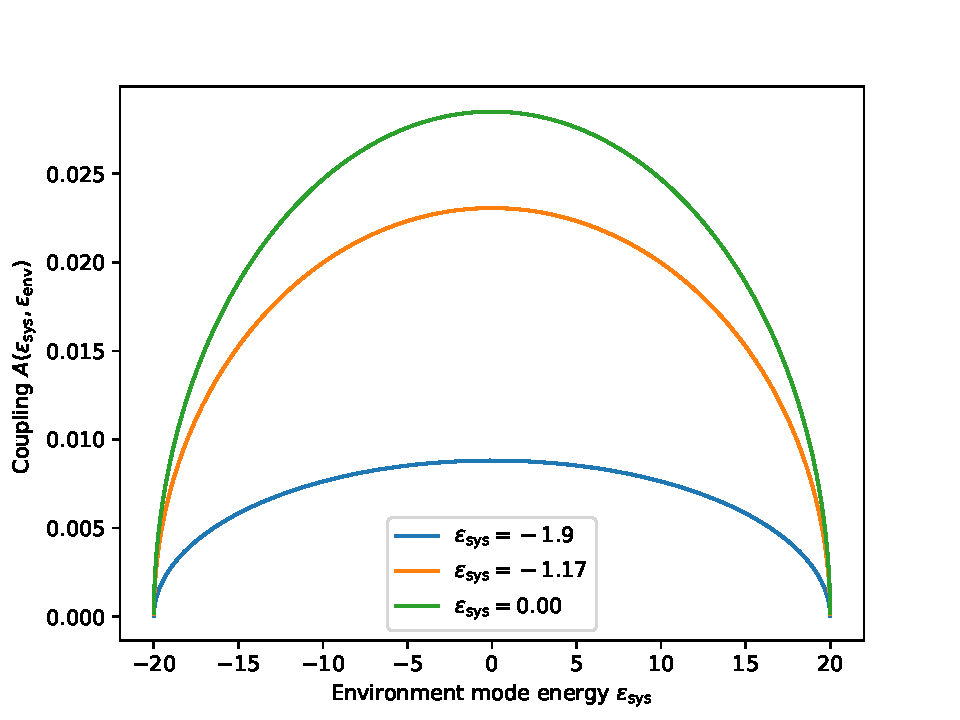
\includegraphics[width=0.9\textwidth]{../plots/Coupling_envModes.pdf}
	\caption{Coupling of different system modes to all environment modes.}\label{fig:Coupling_En_env}
\end{figure}
\section{Energy-dependent coupling in an open quantum system}
The system investigated above allows an unambiguous treatment of the system-environment coupling in real space. Using our analysis, we also showed how individual modes of the environment chain couple to the system modes. However, the discussion has been limited so far to finite systems. To incorporate a truly semi-infinite environment, one has to resort to a different level of theory. The one we will use here is based on the non-equilibrium Green's function formalism, which yields an exact description of the open quantum system. 
The Hamiltonian now reads
\begin{equation}
	H_\mathrm{env} = \sum_k \varepsilon_k c_k^\dagger c_k^\pdagger
\end{equation}
which describes the environment in $k$-space, whereas the system remains unchanged. 
The system-environment coupling is typically taken of the form
\begin{equation}
	H_\mathrm{sys-env} = -\sum_k \gamma_k c_k^\dagger d_{1_\mathrm{sys}} + \mathrm{h.c.}
\end{equation}
which means that the leftmost site of the system couples to all environmental modes with strengths $\gamma_k$\footnote{In fact, this model is related to the partitioned diagonalization introduced above, by transforming the environment  and system-environment Hamiltonians only, while the system Hamiltonian remains unchanged.}. The coupling to the environment is characterized by the level-width (or spectral function) $\Gamma(\varepsilon)$
\begin{equation}
	\Gamma(\varepsilon) = 2\pi \sum_k \gamma_{k}^2\delta(\varepsilon-\varepsilon_k).
\end{equation}
A possible assumption is that $\Gamma(\varepsilon)=\Gamma=\mathrm{const.}$, the so-called wide band limit\footnote{this assumption can be relieved by considering a density of states of the leads $\rho_\mathrm{env}(\varepsilon)$. For this case, the coupling term is $2\pi\gamma^2 \rho_\mathrm{env}(\varepsilon)$.}, which is valid if the bandwidth of the environmental spectrum is larger than the bandwidth of the system. Now, contrary to the coupling introduced before, the level-width function $\Gamma$ takes the form
\begin{equation}
	\Gamma = \begin{pmatrix}
		2\pi \gamma^2 & 0 & \dots & 0\\
		\vdots & & &\vdots\\
		0 & 0 &\dots & 0
	\end{pmatrix}
\end{equation} 
It is straight-forward to obtain the transformed $\Gamma$ in energy-space as the only partition which is still formulated in real-space is the system Hamiltonian. After diagonalizing the system Hamiltonian, again via a unitary $V$, one obtains the coupling $\tilde{\Gamma}$
\begin{equation}
	\tilde{\Gamma} = V^\dagger \Gamma V.
\end{equation}
This transformed coupling is interpreted as the coupling strength of a system mode to all environment modes. 
Going to an open quantum system formalism, we loose all information on the individual environmental modes. \\
\indent \textit{Numerical example}: We consider again a finite system with $L_\mathrm{sys}=21$ sites, with again the leftmost site coupling, now, to all environment modes with equal coupling strength $\gamma$. 
\section{Relation to quantum transport models and validity of partitioned diagonalization beyond the two-chain model}
In a quantum transport setting, one typically considers not only a single environment, but two: One for the source and one for the drain electrode. Here we show that the above analysis cannot be extended to this scenario.
\end{document}




